\documentclass[twoside,twocolumn]{article}

\usepackage{blindtext} 
\usepackage{graphicx}
\usepackage[sc]{mathpazo} 
\usepackage[T1]{fontenc} 
\linespread{1.05} 
\usepackage{microtype} 


\usepackage[english]{babel} 


\usepackage[hmarginratio=1:1,top=32mm,columnsep=20pt]{geometry} 
\usepackage[hang, small,labelfont=bf,up,textfont=it,up]{caption} 
\usepackage{booktabs} 


\usepackage{lettrine} 


\usepackage{enumitem} 
\setlist[itemize]{noitemsep} 


\usepackage{abstract} 
\renewcommand{\abstractnamefont}{\normalfont\bfseries} 
\renewcommand{\abstracttextfont}{\normalfont\small\itshape} 


\usepackage{titlesec} 
\renewcommand\thesection{\Roman{section}} % 
\renewcommand\thesubsection{\roman{subsection}} 
\titleformat{\section}[block]{\large\scshape\centering}{\thesection.}{1em}{} 
\titleformat{\subsection}[block]{\large}{\thesubsection.}{1em}{} 


\usepackage{fancyhdr} 
\pagestyle{fancy} 
\fancyhead{} 
\fancyfoot{} 
\fancyhead[C]{Trabajo de la Unidad$\bullet$ Septienmbre 2020 $\bullet$ } 
\fancyfoot[RO,LE]{\thepage} 


\usepackage{titling} 


\usepackage{hyperref} 
\rmfamily


%----------------------------------------------------------------------------------------
%	TILULOS
%----------------------------------------------------------------------------------------


\setlength{\droptitle}{-4\baselineskip} 

\pretitle{\begin{center}\Huge\bfseries} 
\posttitle{\end{center}} 
\title{Implementación de Call Center y asistencia para el poder judicial} 
\author{Samuel Nuñez Mamani - Franklin Carlos, Huichi Contreras, \\
Anthony Robles Flores. }
\date{\today} 
\renewcommand{\maketitlehookd}{
\begin{abstract}
\noindent 
El presente proyecto pretendió mejorar la calidad de atención de la Corte Superior de Justicia de Tacna y se enfocó en funcionalidades de asistencia y automatización de procesos y/o servicios mediante el uso de tecnologías de información. Se realizó una investigación y análisis de procesos de la institución para delimitar el alcance de esta solución. Se utilizaron herramientas como React Native, Firebase, Voximplant y DialogFlow para la construcción de la solución. Luego de implementar la propuesta, se observó un incremento en la recepción de trámites de la población de la zona y de acuerdo a una encuesta realizada, esta indicaba que un gran porcentaje de usuarios se sentía satisfecho con este canal al poder ahora recibir atención de manera casi inmediata.
\end{abstract}
\begin{abstract}
\noindent 
The present project aimed to improve the quality of attention of the Superior Court of Justice of Tacna and focused on functionalities of assistance and automation of processes and / or services through the use of information technologies. An investigation and analysis of the institution's processes was carried out to define the scope of this solution. Tools such as React Native, Firebase, Voximplant and DialogFlow were used to build the solution. After implementing the proposal, an increase in the reception of procedures from the population of the area was observed and according to a survey carried out, this indicated that a large percentage of users felt satisfied with this channel as they can now receive attention in a manner almost immediate.

\end{abstract}
}

%----------------------------------------------------------------------------------------

\begin{document}

% Print the title
\maketitle

%----------------------------------------------------------------------------------------
%	INTRODUCCION
%----------------------------------------------------------------------------------------

\section{Introduccion}
Los centros de llamadas operadas o de contacto  hoy en dia por personal es una proveedora de servicios que se encarga de dar soporte y administrar dependiendo los servicios o solicitudes que las empresas proveen. Estos Centros de contactos normalmente son operados en instalaciones que cuentan con equipos como computadoras, telefonos, microfonos,etc. Estos centros suelen estar conectados con algun otro centro o tambien son prestadoras de servicios de estaciones ya establecidas.\\
Actualmente las mas reconocidas e importantes empresas usan centros de contacto para realizar una interaccion con los clientes entre ellos podemos 
contar firmas para pedidos por catalogo, soportes operativos, atencion al cliente, etc.

\section{Planteamiento del problema}
\subsection{Descripcion del problema}
En el poder judicial se reciben constantes llamadas de parte del publico la cual buscan resolver problema que involucran con la institucion, el problema nace cuando el personal que atiende
el problema no es el calificado para resolverla y este lo redirecciona a otra persona y de esta manera el solicitante se queda buscando a alguien que pueda resolver esta duda haciendo de
esta una experiencia lenta y tediosa.

\subsection{Formulación del problema}
\subsubsection{General}
¿Lograra un call center mediante un asistente virtual resolver las consultas de los clientes ?

\subsection{Justificacion}
El proyecto que a continuación se presenta, no sólo busca responder las consultas del publico solicitante, sino espera lograr,
a través de la tecnología, la automatizacion de consultas extras que puedan ser facilmente contestadas aprovechando el servicio implementado.
La finalidad principal de éste proyecto es aportar una solución tecnológica de corto y largo plazo para un proceso que mejore la atencion al cliente
dentro del Poder Judicial.

\subsection{Alcance}
El alcance final del trabajo será lograr implementar un
software que logre mejorar la atencion de las personas que tengan dudas o consultas acerca del Poder Judicial, siendo estas capaces de responder.

\section{Objetivos}
\subsection{General}
Mejorar la calidad de atención de la Corte Superior de Justicia de Tacna a la población

\subsection{Especificos}
\begin{itemize}
\item Establecer un canal de comunicación por voz automatizado que responda a las solicitudes de las personas.
\item Procesar la mayor cantidad de solicitudes.
\item Resolver consultas inmediatas que no requieran de apersonarse a la institución.
\end{itemize}

\section{Descripcíon del Proyecto}
\subsection{Problemática}
Actualmente a nivel Mundial la aparición del Covid19 a provocado un desorden Global, para que este virus no se propague, nuestro Gobierno fue obligado a decretar un "Estado de Emergencia" a nivel nacional provocando asi una paralización brusca en la gran mayoría de trabajos.
\\
Esto provocó un adaptamiento brusco a continuar con las jornadas laborales pero de forma virtual , utilizando asi todos los canales de comunicación posibles.
El personal de muchas organizaciones pasaron de sus jornadas agregando un plus extra el cual es estar pendiente en todos los canales de comunicación para el usuario.
\\
El Poder Judicial de Tacna, atraviesa esta situación provocando que las jornadas sean presenciales y virtuales, sumándole a esto una saturación constante de llamadas de   interrogantes existentes por parte del usuario provocando asi un retraso en sus actividades cotidianas y también una molestia constante por la gran cantidad de llamadas entrantes a su respectivo anexo como resultado llevarlos a un cuadro de estrés que en un futuro podría perjudicarles en su labores.

\subsection{Propuesta de Solución}
Para solucionar esta problemática existente en el poder judicial tomando en cuenta estos tiempos de la pandemia donde el asilamiento social a provocado un desbalance en las actividades normales de los trabajadores en esta entidad sobrecargando con labores adicionales para el proceso de adaptamiento a este contexto en el que vivimos , la implementacion de un Call Center podría agilizar los procesos de los trabajadores donde un asistente podria solucionar las interrogantes que podrian tener los usuarios antes que un trabajador interno pueda intervenir, pero en caso el asistente no pudiese resolver esta duda , el mismo call center podria derivar a un anexo a poder comunicarse vía telefonica con un asesor legal.
\\
Viendo que existen diferentes canales de comunicación,  en el momento de interactuar con el usuario , proponemos tambien una aplicacion Móvil en Android donde este prodrá otorgar los mismos servicios añadiendo tambien la facilidad al usuario de poder ubicar las oficinas de acuerdo a la sucursal en la que necesiter asistir a una cita programada , como tambien  el llenado de formularios con formatos ya establecidos por el poder judicial donde hay algunos documetos que no se necesiten la evaluacion de un abogado y como resultado la aplicacion podría descargar un PDF con los datos solicitados usando el formato de documentos del Poder Judicial.
\\
Tomando en cuenta que la tecnologia de tener un SmartPhone invade cada vez mas a la sociedad , incluir un módulo en el aplicativo acerca de las audiencias que el poder judicial publicará asi el usuario externo podría tener a la mano esta información a fin de poder asistir y estar pendientes puesto que en la web se encuentra el cronograma pero ubicar una audiencia para aquellos que desconocen el uso de una plataforma web podria ser dificultoso , la aplicacion movil podria ayudar a que sera mas sencillo y rápido de identificar una audiencia.

\subsection{Tecnología de información}
En esta seccion definiremos las herramientas que se utilizaran para el desarrollo del proyecto asi mismos las plataformas que se emplearan para las conexiones en algunos servicios.
\begin{itemize}
\item Plataforma Colaborativa
\subitem Github : Una herramienta colaborativa muy útil en el control de versiones para el desarrollo de un Proyecto de Software con la capacidad de poder crear ramas para el crecimiento en escala de menor a mayor de un Sistema.
\subitem Google Meet : Una aplicación de videoconferencia que permitirá a los integrantes de grupo poder entablar una comunicación virtual para poder facilitar el trabajo en equipo.
\subitem Teams Microsoft : Plan de contigencia en caso el Google meet pueda caer, puede ser usado puesto que la propia Universidad Privada de Tacna puede otorgar a los estudiantes para realizar videconferencias interactivas con los integrantes del grupo de proyecto con múltiples herramientas que ayudarán para la colaboracion en la elaboración de este proyecto.
\item Base de Datos:
\subitem Firebase RealTime DataBase : Nos permitirá sincronizar datos con nuestra Base de Datos NoSQL alojada en la nube, estos datos se sincronizaran con todos los clientes en tiempo real.
\item Lenguajes de programación:
\subitem Lenguaje Java.
\item Entorno de Desarrollo:
\subitem Android Studio : Entorno que nos permitirá desarrollar aplicaciones móviles.
\item Asistente Virtual:
\subitem DialogFlow : Plataforma que nos permitirá agentes virtuales o asistentes virtuales para una futura integración en multiples canales de comunicación.
\item Red Telefonica:
\subitem VoximPlant.
\end{itemize}

\subsection{Arquitectura del Call Center}

\begin{figure}[h!]
	\begin{center}
		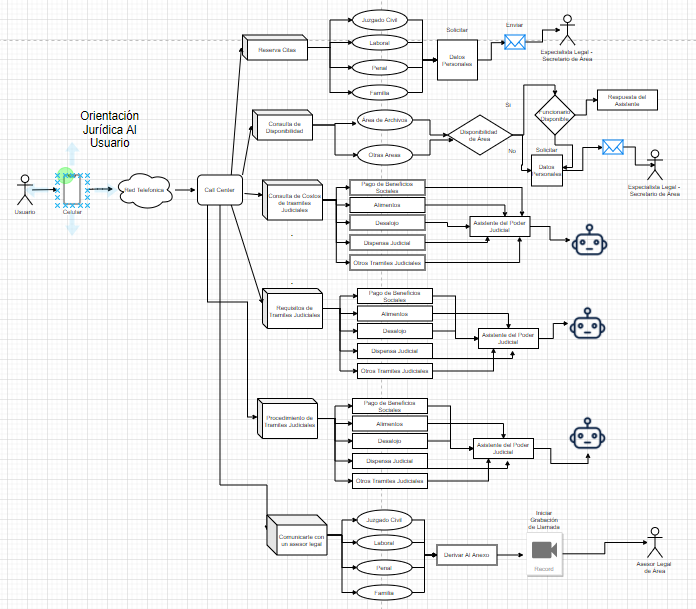
\includegraphics[width=7.5cm]{./Imagenes/callcenter} 
		\caption{Call Center}
	\end{center}
\end{figure}


\subsection{Metodología}
La metodologia que usaremos será RUP (Proceso Unificado de Rational)puesto que esta metodología provee un entorno de desarrollo flexible basado en estándares que se adapta a las necesidades del desarrollador o de las empresas y tener la facilidad de dividir todas las actividades de forma de que a cada participantele pueda tocar la parte que le compete.
\subsection{Arquitectura de la Aplicación}

\begin{figure}[h!]
	\begin{center}
		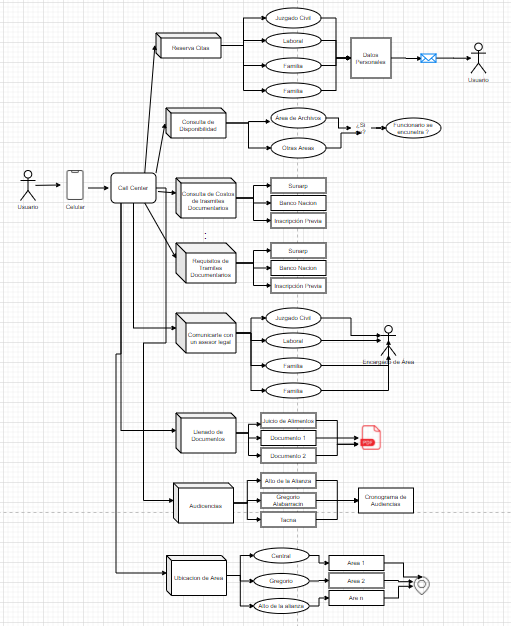
\includegraphics[width=7.5cm]{./Imagenes/apk} 
		\caption{Aplicación Movil}
	\end{center}
\end{figure}

\section{Resultados}

Entre los hallazgos más destacables se notó que 

\section{Conclusiones}
Con los resultados expuestos observamos que el empleo oportuno de tecnologías de información como los bots y asistentes virtuales demuestran tener bastante potencial para contribuir a la mejora y alza de movimiento en los procesos de un negocio, en este caso de la Corte Superior de Justicia de Tacna.

\end{document}
